\subsection{Factored form}

We will now evaluate the evaluation precision of the following factored rewriting:
\[
    T(x) = 1 + 8x^2\,(x-1)\,(x+1)\,(4x^2 + 2x - 1)^2\, (4x^2 - 2x - 1)^2\,(16x^4 - 20x^2 + 5)^2
\]

\begin{eqnarray*}
    T(x) &=& 8.0*x^2*(x - 1.0)*(x + 1.0) \\
    & & * (4.0*x^2 + 2.0*x - 1.0)*(4.0*x^2 + 2.0*x - 1.0) \\
    & & * (4.0*x^2 - 2.0*x - 1.0)*(4.0*x^2 - 2.0*x - 1.0)* \\
    & & * (16.0*x^4 - 20.0*x^2 + 5.0)*(16.0*x^4 - 20.0*x^2 + 5.0) + 1 \\
\end{eqnarray*}

\begin{question}
    \begin{enumerate}[(a)]
        \item Open the file {\tt tchebychev.c} and have a look to the function {\tt REAL factored (REAL x)}
        \item Execute the command {\tt ./run.sh FACTORED FLOAT 24} \newline
              The output of this command is given in figure~\ref{fig:factored:float}.
        \item Compare these results to those obtained with the EXPANDED version.
    \end{enumerate}
\end{question}

\begin{figure}[h]
    \center 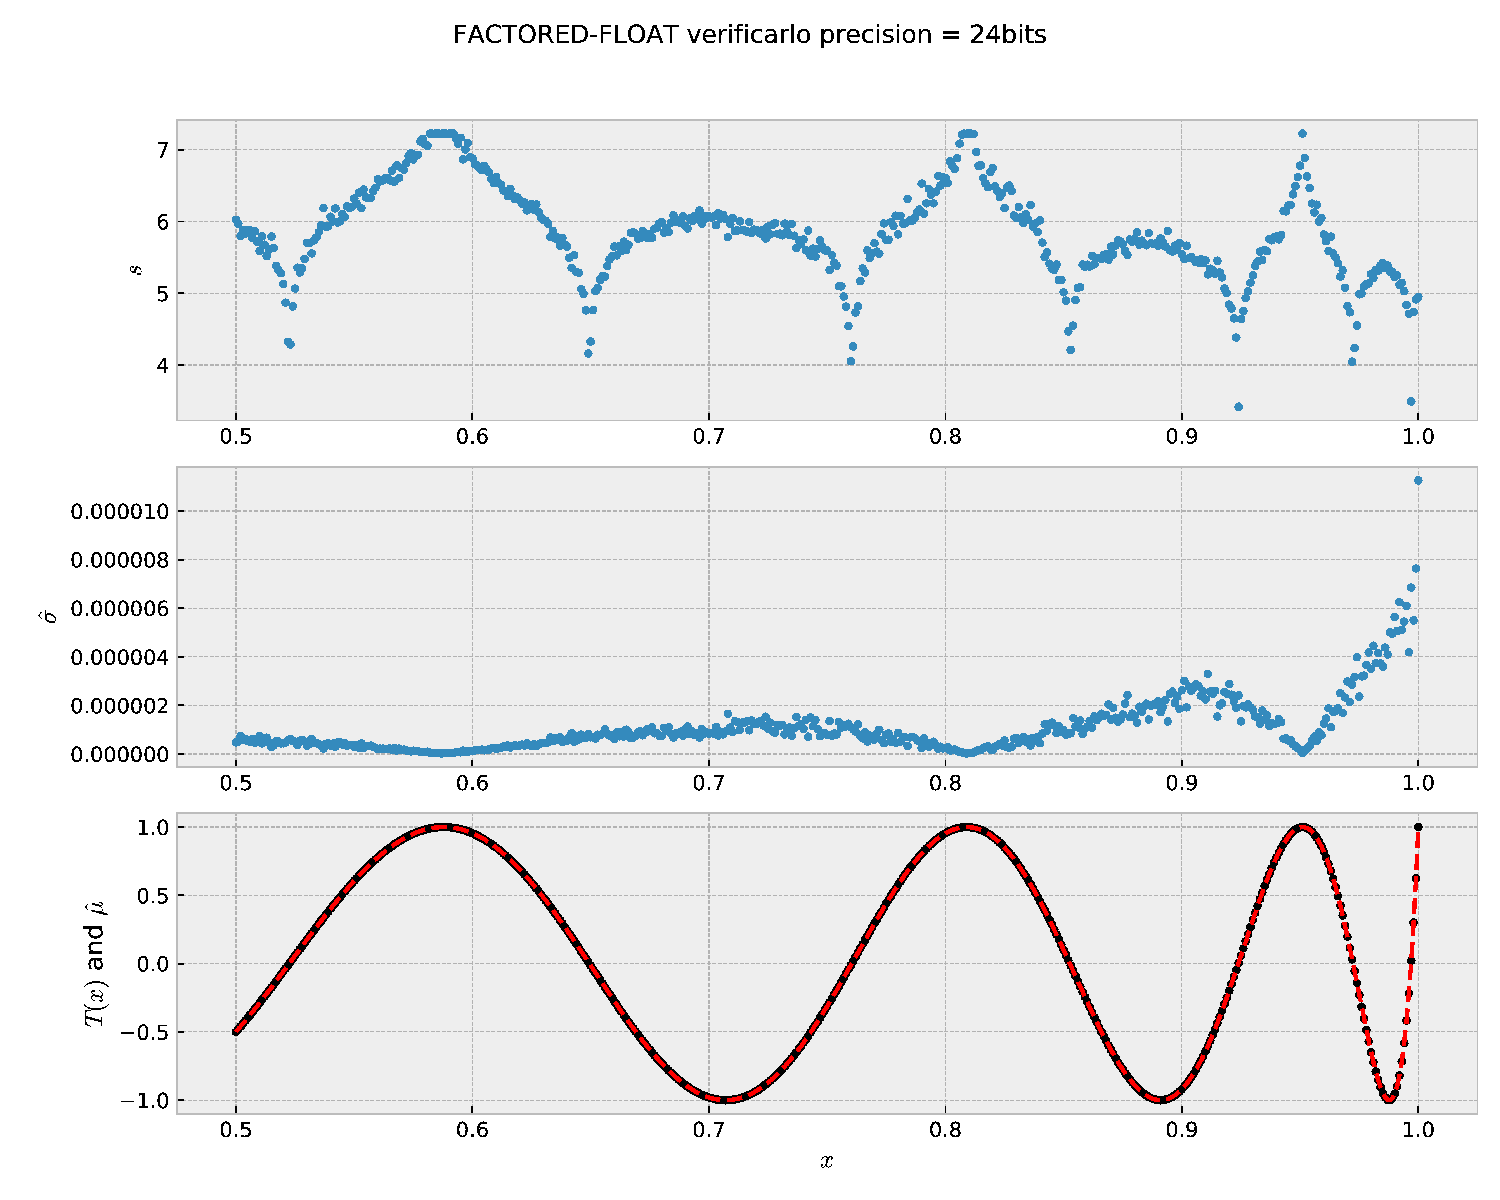
\includegraphics[width=.8\textwidth]{FACTORED-FLOAT-24.pdf}
    \caption{Evaluation of T(x) in its factored form, compiled in single precision, with a virtual precision of 24}
    \label{fig:factored:float}
\end{figure}

\begin{question}
    Explain what happens when $T(x)=1$ for $x\simeq 0.6$,
    $x\simeq 0.8$ et $x\simeq 0.95$.\\~\\
    $\rightarrow$ We evaluate $T$ on one of the roots of the factored right-hand terms which become zero.
    It is an example where the error is absorbed and the precision and accuracy of the results are improved.
\end{question}


%\begin{question}
%  \begin{enumerate}[(a)]
%    \item Modify the {\tt run.sh} script to evaluate the  polynomial between $0.99$ and $1$ by $0.00001$ step.
%    \item Run the scripts to execute and visualize the results for
%          FACTORED, EXPANDED and HORNER with a virtual precision of 53. The results are respectively presented in figure~\ref{fig:factored:double:53:zoom},\ref{fig:expanded:double:53:zoom}
%          and~\ref{fig:horner:double:53:zoom}.
%
%    \item Reproduce the result with a virtual precision of 24. The results are respectively presented in figure~\ref{fig:factored:double:24:zoom},\ref{fig:expanded:double:24:zoom}
%          and~\ref{fig:horner:double:24:zoom}
%
%  \end{enumerate}
%\end{question}
%
%\begin{figure}[h]
%  \center 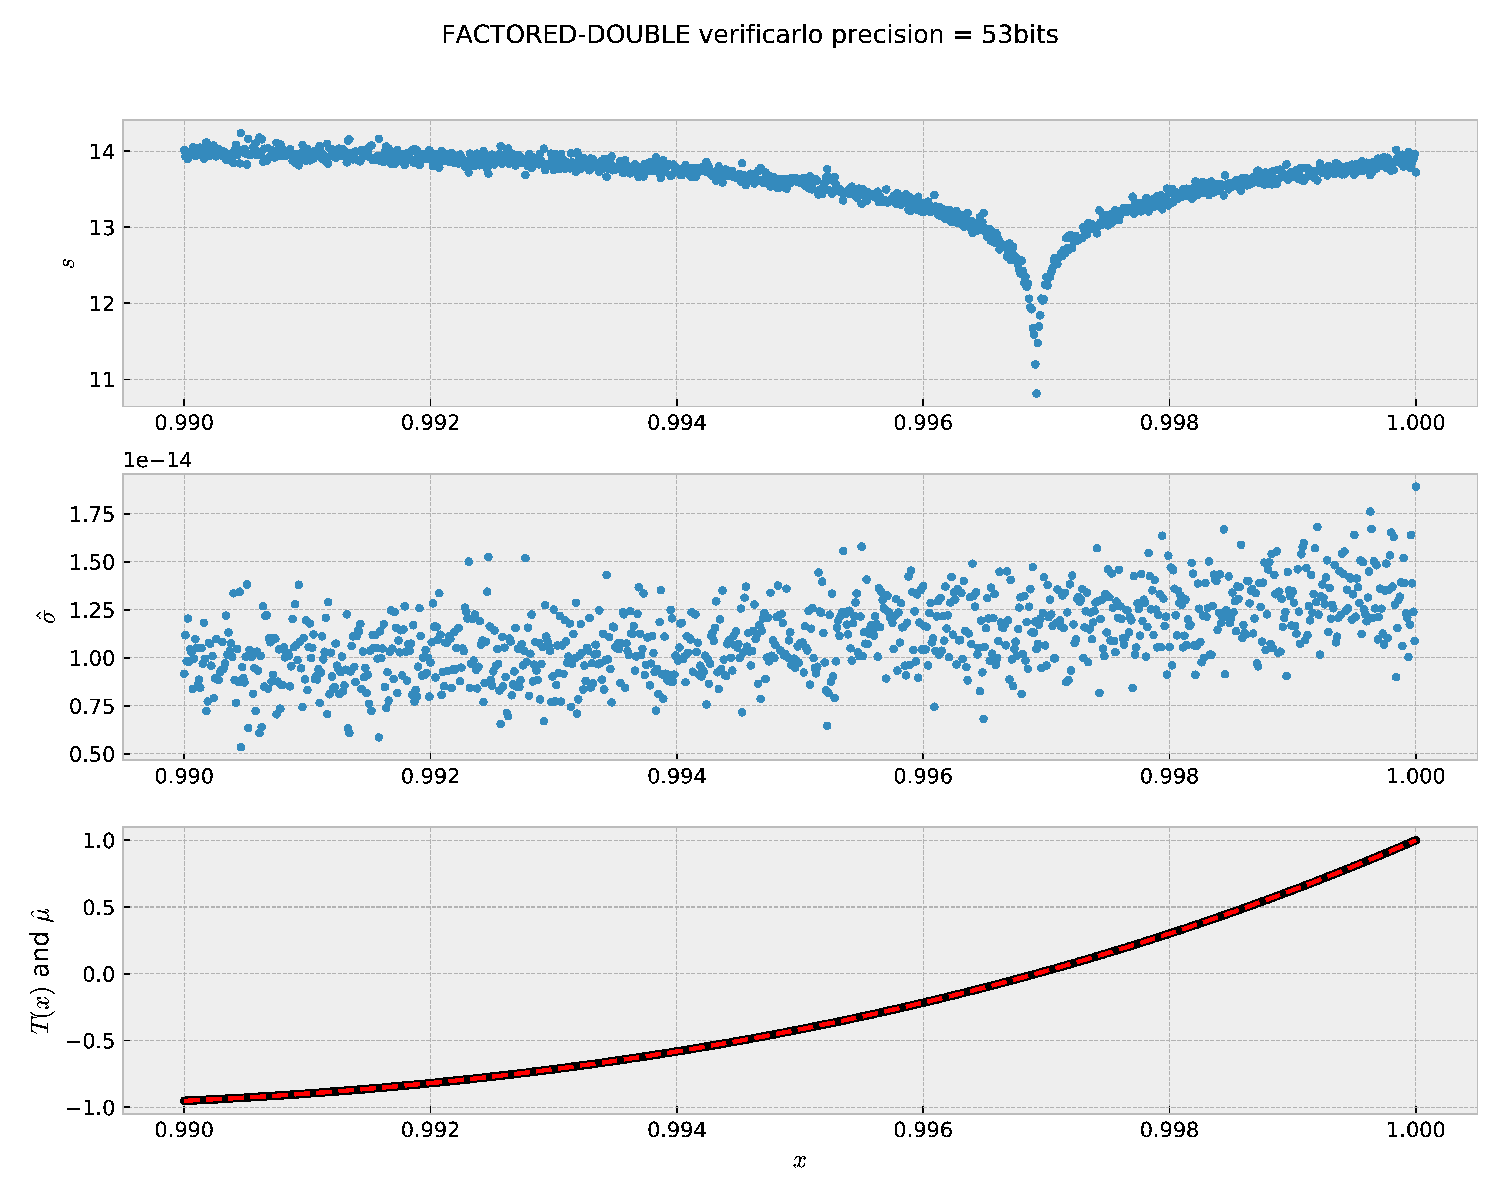
\includegraphics[width=.8\textwidth]{FACTORED-DOUBLE-53-zoom.pdf}
%  \caption{Evaluation of T(x) in its factored form, compiled in double
%    precision, with a virtual precision of 53}
%  \label{fig:factored:double:53:zoom}
%\end{figure}

%\begin{figure}[h]
%  \center 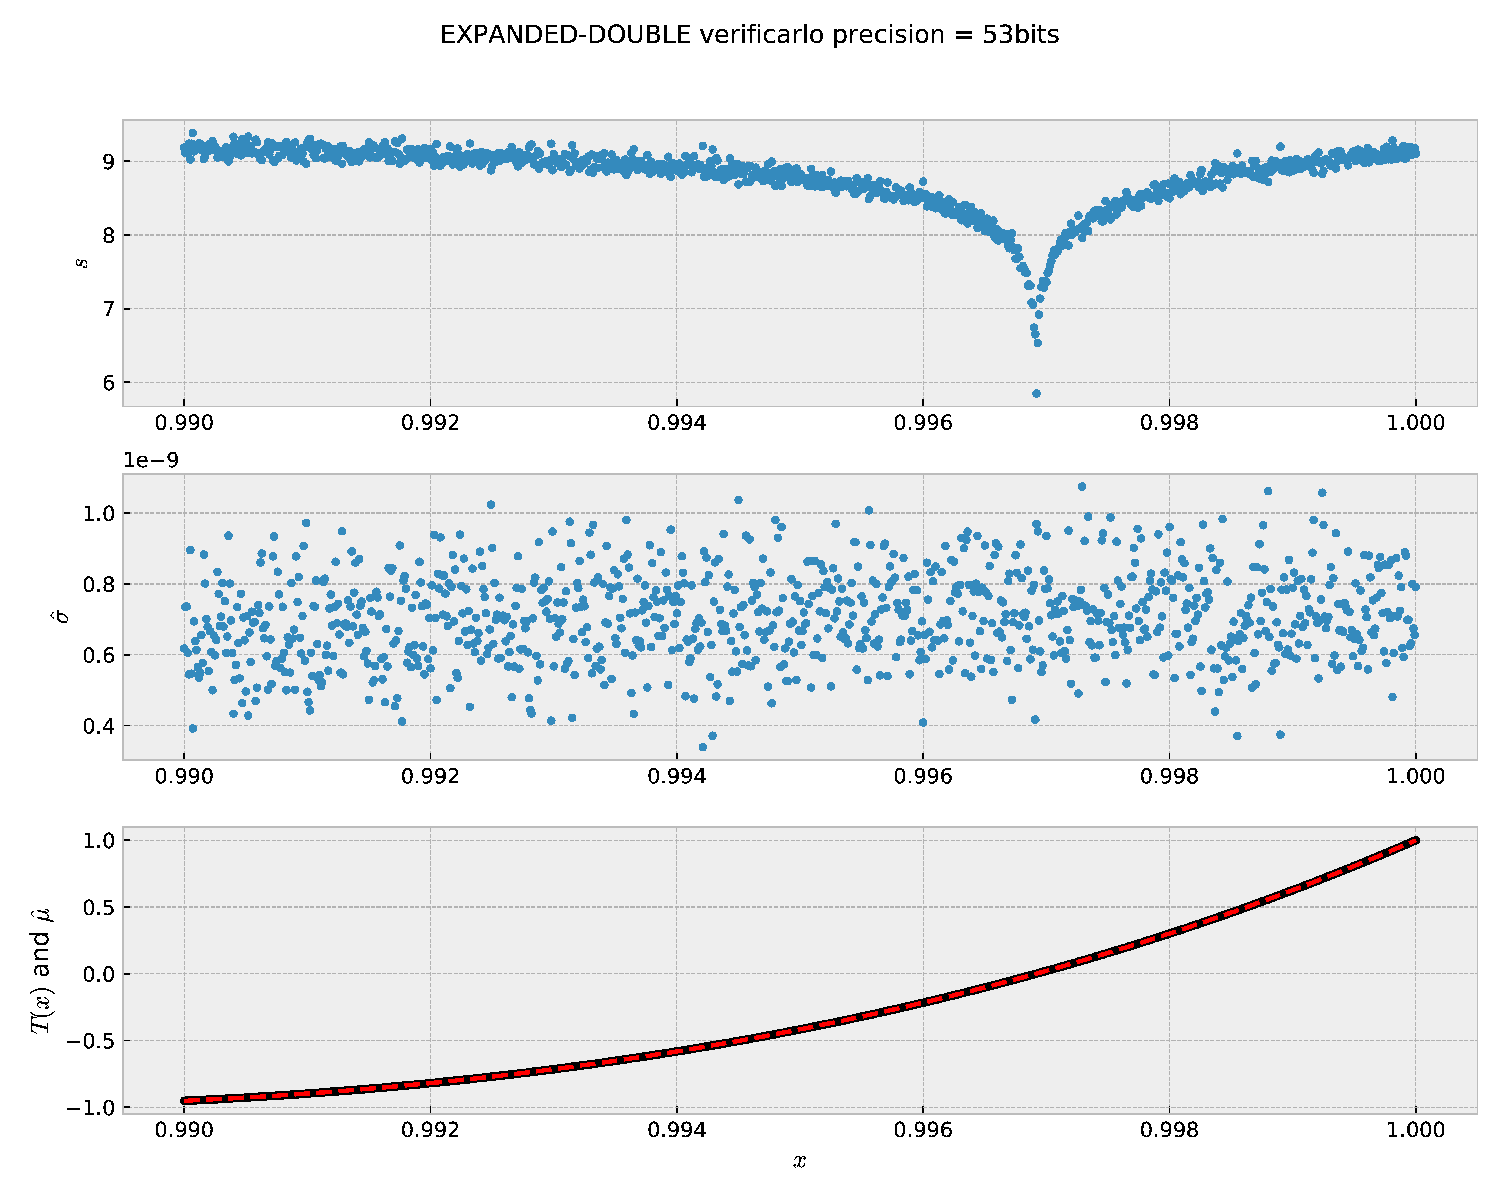
\includegraphics[width=.8\textwidth]{EXPANDED-DOUBLE-53-zoom.pdf}
%  \caption{Evaluation of T(x) in its expanded form, compiled in double
%    precision, with a virtual precision of 53}
%  \label{fig:expanded:double:53:zoom}
%\end{figure}
%
%\begin{figure}[h]
%  \center 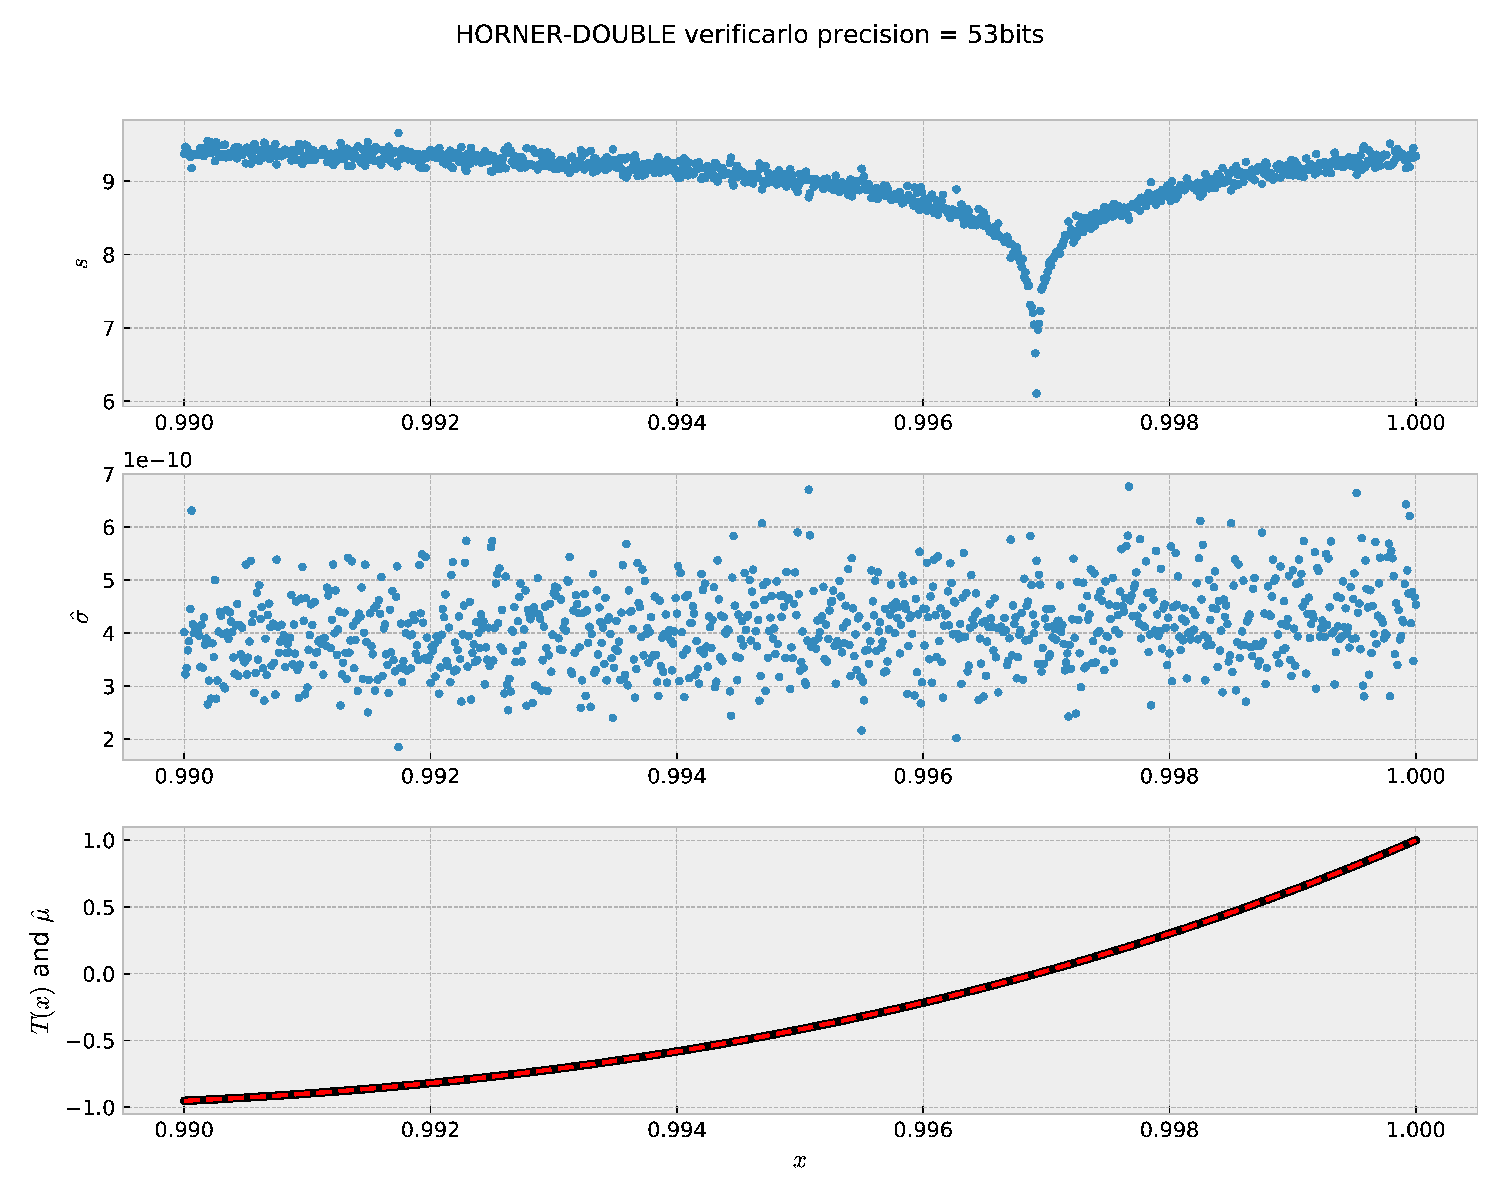
\includegraphics[width=.8\textwidth]{HORNER-DOUBLE-53-zoom.pdf}
%  \caption{Evaluation of T(x) using Horner scheme, compiled in double precision,
%    with a virtual precision of 53}
%  \label{fig:horner:double:53:zoom}
%\end{figure}
%
%\begin{figure}[h]
%  \center 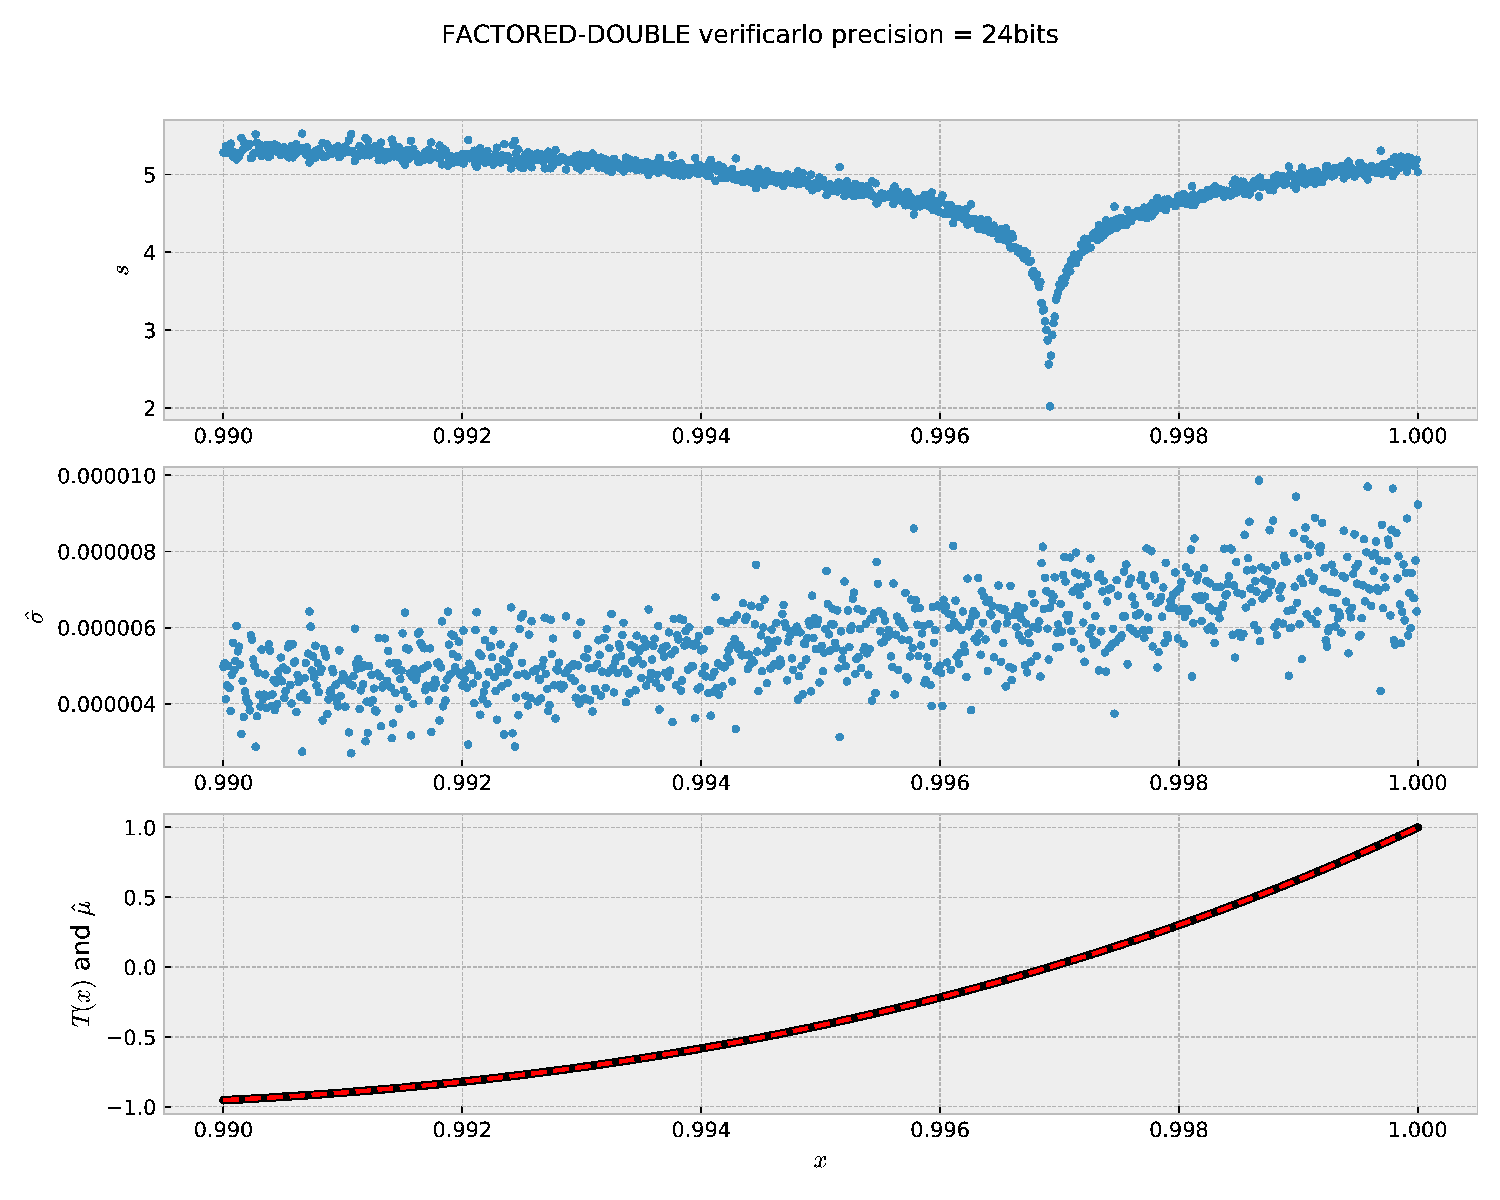
\includegraphics[width=.8\textwidth]{FACTORED-DOUBLE-24-zoom.pdf}
%  \caption{Evaluation of T(x) in its factored form, compiled in double
%    precision, with a virtual precision of 24}
%  \label{fig:factored:double:24:zoom}
%\end{figure}
%
%\begin{figure}[h]
%  \center 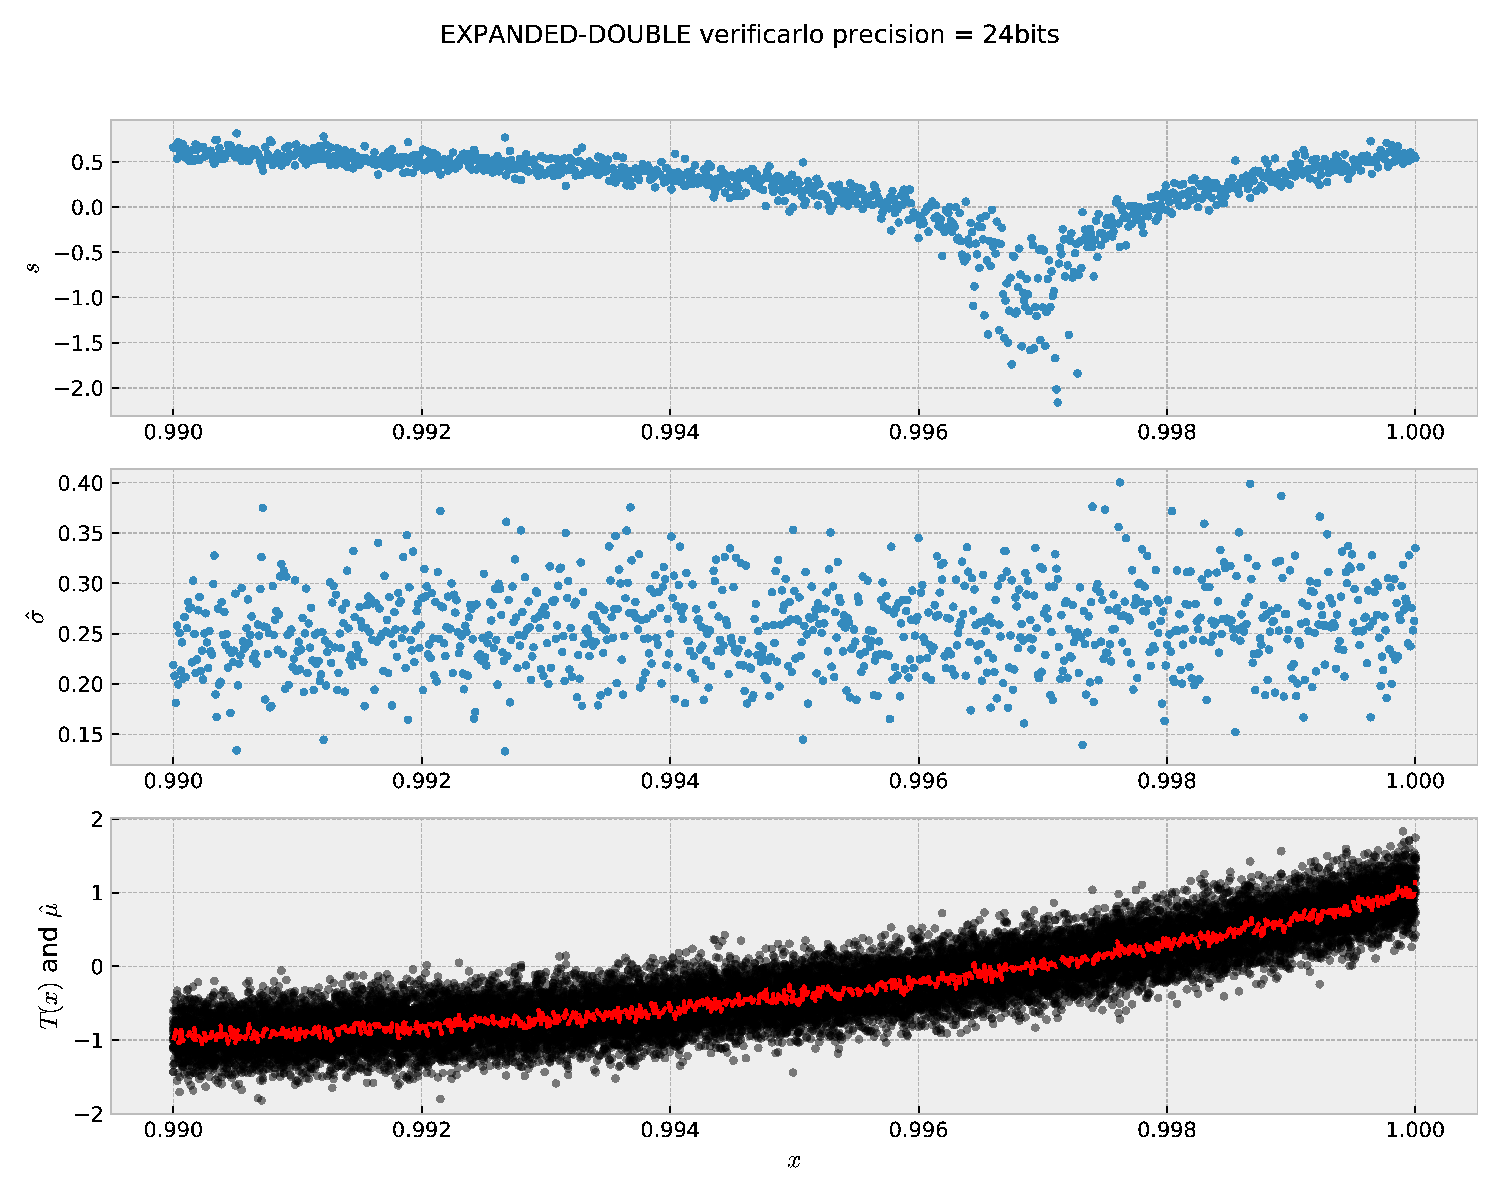
\includegraphics[width=.8\textwidth]{EXPANDED-DOUBLE-24-zoom.pdf}
%  \caption{Evaluation of T(x) in its expanded form, compiled in double
%    precision, with a virtual precision of 24}
%  \label{fig:expanded:double:24:zoom}
%\end{figure}
%
%\begin{figure}[h]
%  \center 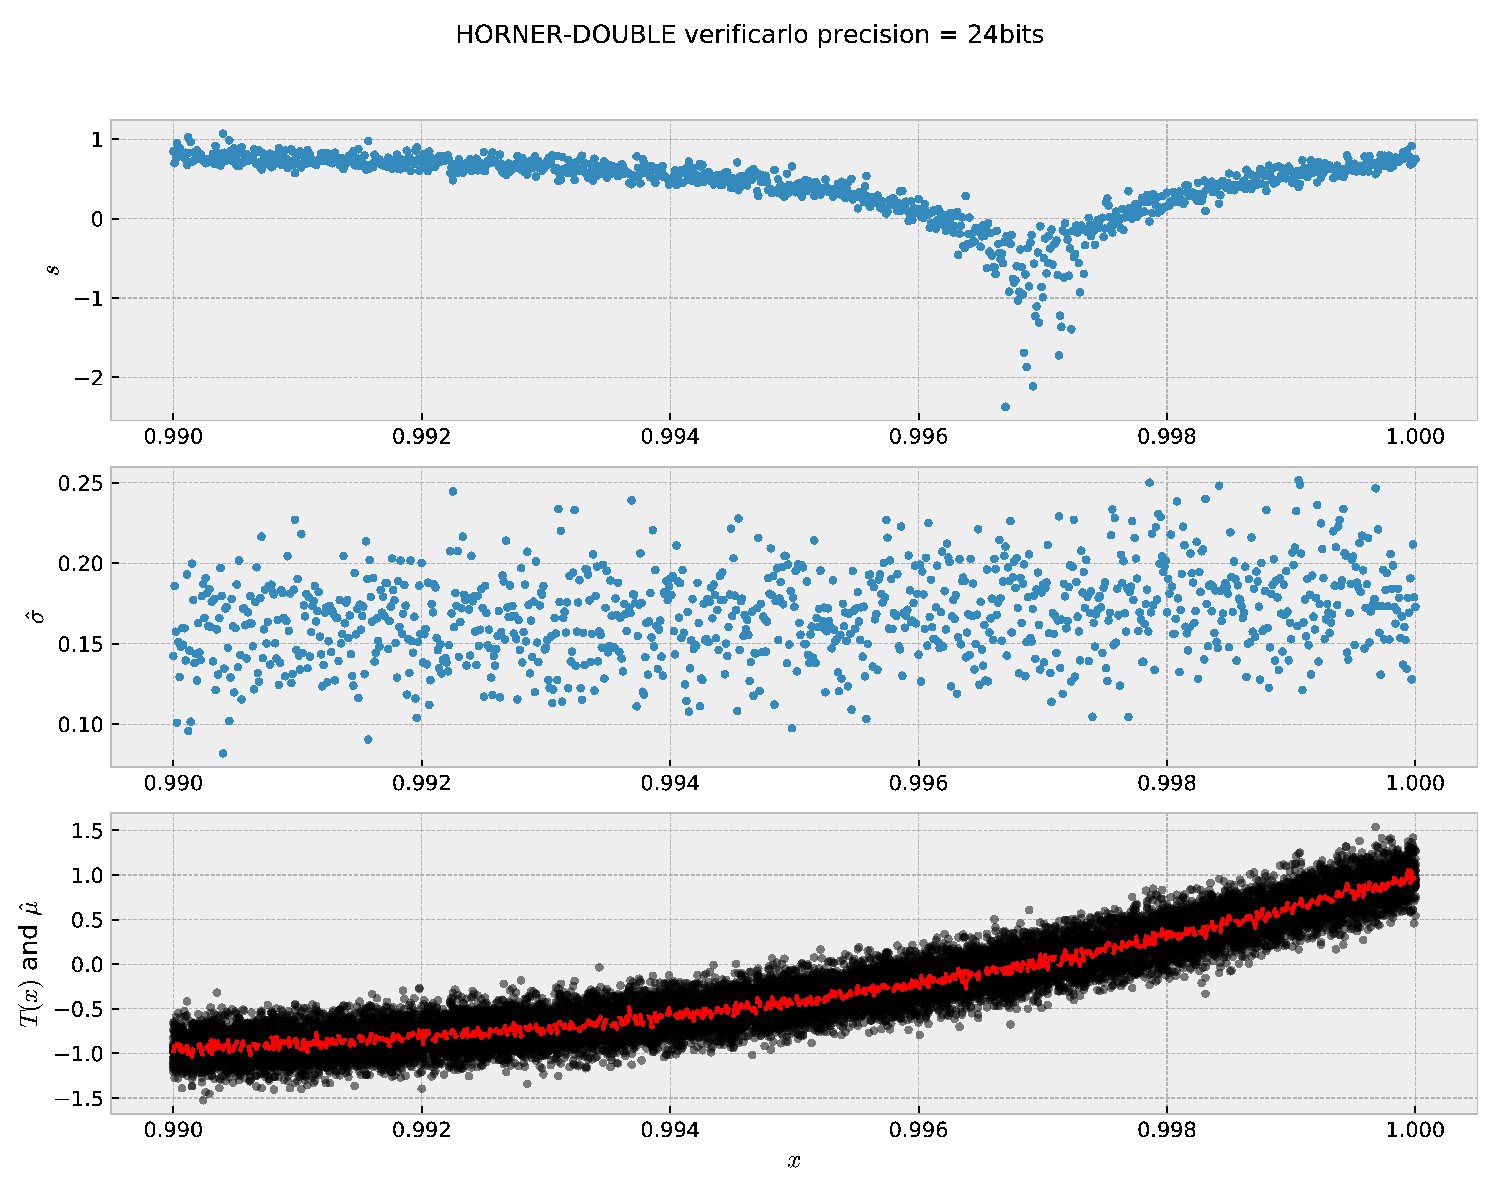
\includegraphics[width=.8\textwidth]{HORNER-DOUBLE-24-zoom.pdf}
%  \caption{Evaluation of T(x) using Horner scheme, compiled in double precision,
%    with a virtual precision of 24}
%  \label{fig:horner:double:24:zoom}
%\end{figure}

\section{VPREC: Variable precision backend}

The VPREC backend emulates reduced floating-point formats without having to
change the implementation. It can emulate any format that fits into the original
type. Unlike the MCA backend, VPREC is deterministic. It mirrors what would happen
with the selected reduced type. It correctly handles overflow, underflows, and
rounding in the target type.

To use VPREC one can either tune manually the range and precision of the target
type. The option {\tt --precision-binary64=PRECISION} controls the
pseudo-mantissa bit length of the new tested format for floating-point
operations in double precision. The option {\tt --range-binary64=PRECISION}
controls the exponent bit length of the target format.

One can also use one of the standard presets: binary16, binary32, bfloat16,
tensorfloat, fp24, PXR24; which automatically sets the corresponding range and
precisions. The option for setting a preset is {\tt --preset=PRESET}.


\begin{question}
    \begin{enumerate}[(a)]
        \item Compile and run the benchmark using single precision without verificarlo
              \begin{verbatim}
clang -D FLOAT -o reference tchebychev.c
./reference 0.6 FACTORED
6.0000002e-01 9.5425093e-01
\end{verbatim}
        \item Now compile it using double precision with verificarlo
              \begin{verbatim}
verificarlo -D DOUBLE -o tchebychev tchebychev.c
VFC_BACKENDS="libinterflop_vprec.so --preset=binary32" ./tchebychev 0.6 FACTORED 
5.9999999999999998e-01 9.5425069332122803e-01
\end{verbatim}
        \item Compare the mantissas between the two previous runs. Observe that VPREC has accurately emulated binary32 (FLOAT) format.
    \end{enumerate}
\end{question}

\begin{question}
    \begin{enumerate}[(a)]
        \item You can emulate the effect of bfloat16 using
              \begin{verbatim}
VFC_BACKENDS="libinterflop_vprec.so --preset=bfloat16" ./tchebychev 0.6 FACTORED 
5.9999999999999998e-01 9.5312500000000000e-01
\end{verbatim}
        \item You can also emulate a custom precision, such as 10 bits, with
              \begin{verbatim}
VFC_BACKENDS="libinterflop_vprec.so --precision-binary64=10" ./tchebychev 0.6 FACTORED 
5.9999999999999998e-01 9.5263671875000000e-01
\end{verbatim}
        \item Try different precisions, at which threshold does the computation looses all significance ?
    \end{enumerate}
\end{question}

\begin{question}
    \begin{enumerate}[(a)]
        \item Analyze the script {\tt run\_vprec.sh}. This script allows you to plot the result of VPREC runs in the interval $[0.5,1]$.
        \item Use the script to simulate and plot the effect of running FACTORED and EXPANDED versions with bfloat16.
    \end{enumerate}
\end{question}
